\chapter{Wstęp}

\section{Wprowadzenie}

W ostatnich latach technologia blockchain zyskała na znaczeniu, stając się fundamentem rozwoju rynków finansowych oraz innowacji w obszarze kryptowalut. Blockchain, początkowo kojarzony głównie z Bitcoinem, obecnie znajduje szerokie zastosowanie w wielu dziedzinach, od logistyki po usługi bankowe. Jest on technologią rozproszoną, umożliwiającą bezpieczne i~przejrzyste przechowywanie oraz przesyłanie danych bez potrzeby pośredników. Dzięki takim cechom jak decentralizacja i niezaprzeczalność danych, blockchain przyciąga uwagę zarówno instytucji finansowych, jak i indywidualnych użytkowników.

Jedną z najważniejszych zalet blockchaina jest możliwość eliminacji problemu zaufania pomiędzy stronami transakcji. Dzięki transparentności rejestru, blockchain pozwala na przeprowadzanie transakcji między stronami, które nie muszą sobie wzajemnie ufać. Każda operacja jest potwierdzana i zapisywana w sposób niezmienny, co eliminuje ryzyko oszustwa lub manipulacji danymi. Jak zauważył Satoshi Nakamoto, twórca Bitcoina: „Potrzebujemy systemu płatności opierającego się na dowodach kryptograficznych zamiast zaufania, umożliwiającego dwóm dowolnym stronom bezpośrednie przeprowadzanie transakcji bez konieczności korzystania z zaufanej strony trzeciej.”~\cite{nakamoto_2008}.

Rozwój technologii blockchain doprowadził do powstania nowej generacji aplikacji zdecentralizowanych, które mają potencjał zmienić sposób, w jaki funkcjonują instytucje publiczne i~prywatne. Projekty takie jak Ethereum wprowadziły koncepcję smart kontraktów, umożliwiając automatyzację procesów biznesowych i prawnych bez potrzeby angażowania pośredników. Smart kontrakty, działając jako programowalne umowy, pozwalają na realizację warunków zawartych w kodzie, co dodatkowo wzmacnia bezpieczeństwo i przejrzystość transakcji.

Technologia ta znajduje zastosowanie nie tylko w finansach, ale również w innych obszarach, jak łańcuchy dostaw, gdzie umożliwia śledzenie produktów od momentu produkcji aż po finalnego odbiorcę, czy w ochronie zdrowia, zapewniając bezpieczne i anonimowe przechowywanie danych medycznych. Jak zauważa Nakamoto: „Największym problemem tradycyjnych walut jest zaufanie potrzebne do ich funkcjonowania. Bank centralny musi być wiarygodny, aby nie obniżał wartości waluty, ale historia tradycyjnych walut jest pełna naruszeń tego zaufania.”~\cite{nakamoto_2008}.

\begin{figure}[htb]
    \centering
    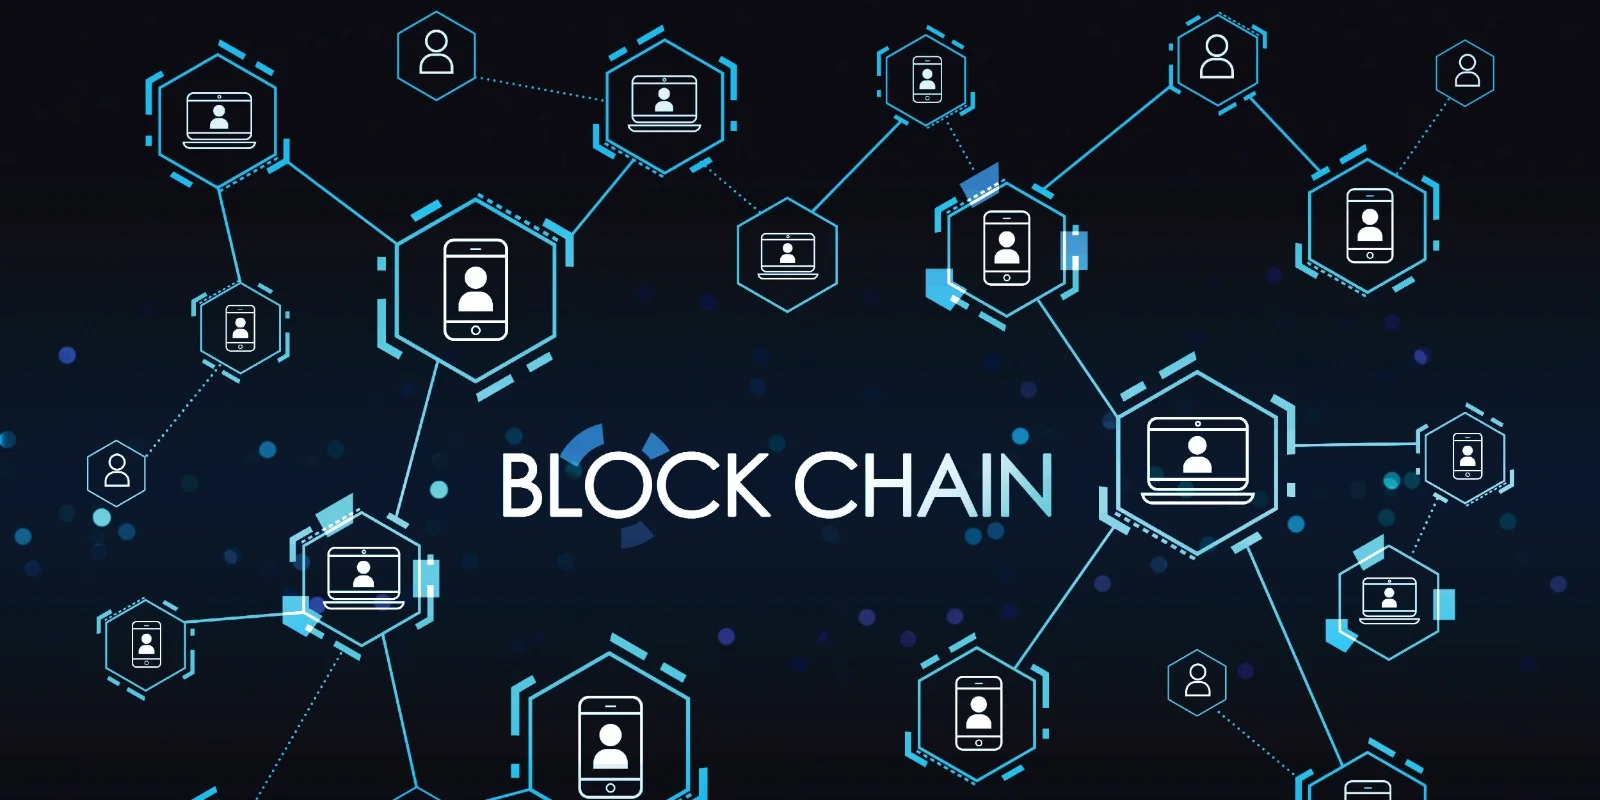
\includegraphics[width=0.8\linewidth]{./obrazy/blockchain}
    \caption{Blockchain}
    \label{fig:Blockchain}
\end{figure}

Mimo potencjału technologii, użytkownicy często napotykają trudności w dostępie do danych z różnych blockchainów oraz ich interpretacji. Istniejące narzędzia, takie jak Etherscan dla Ethereum czy Solscan dla Solany, są przypisane konkretnym sieciom, co ogranicza ich uniwersalność. 
\begin{figure}[htb]
    \centering
    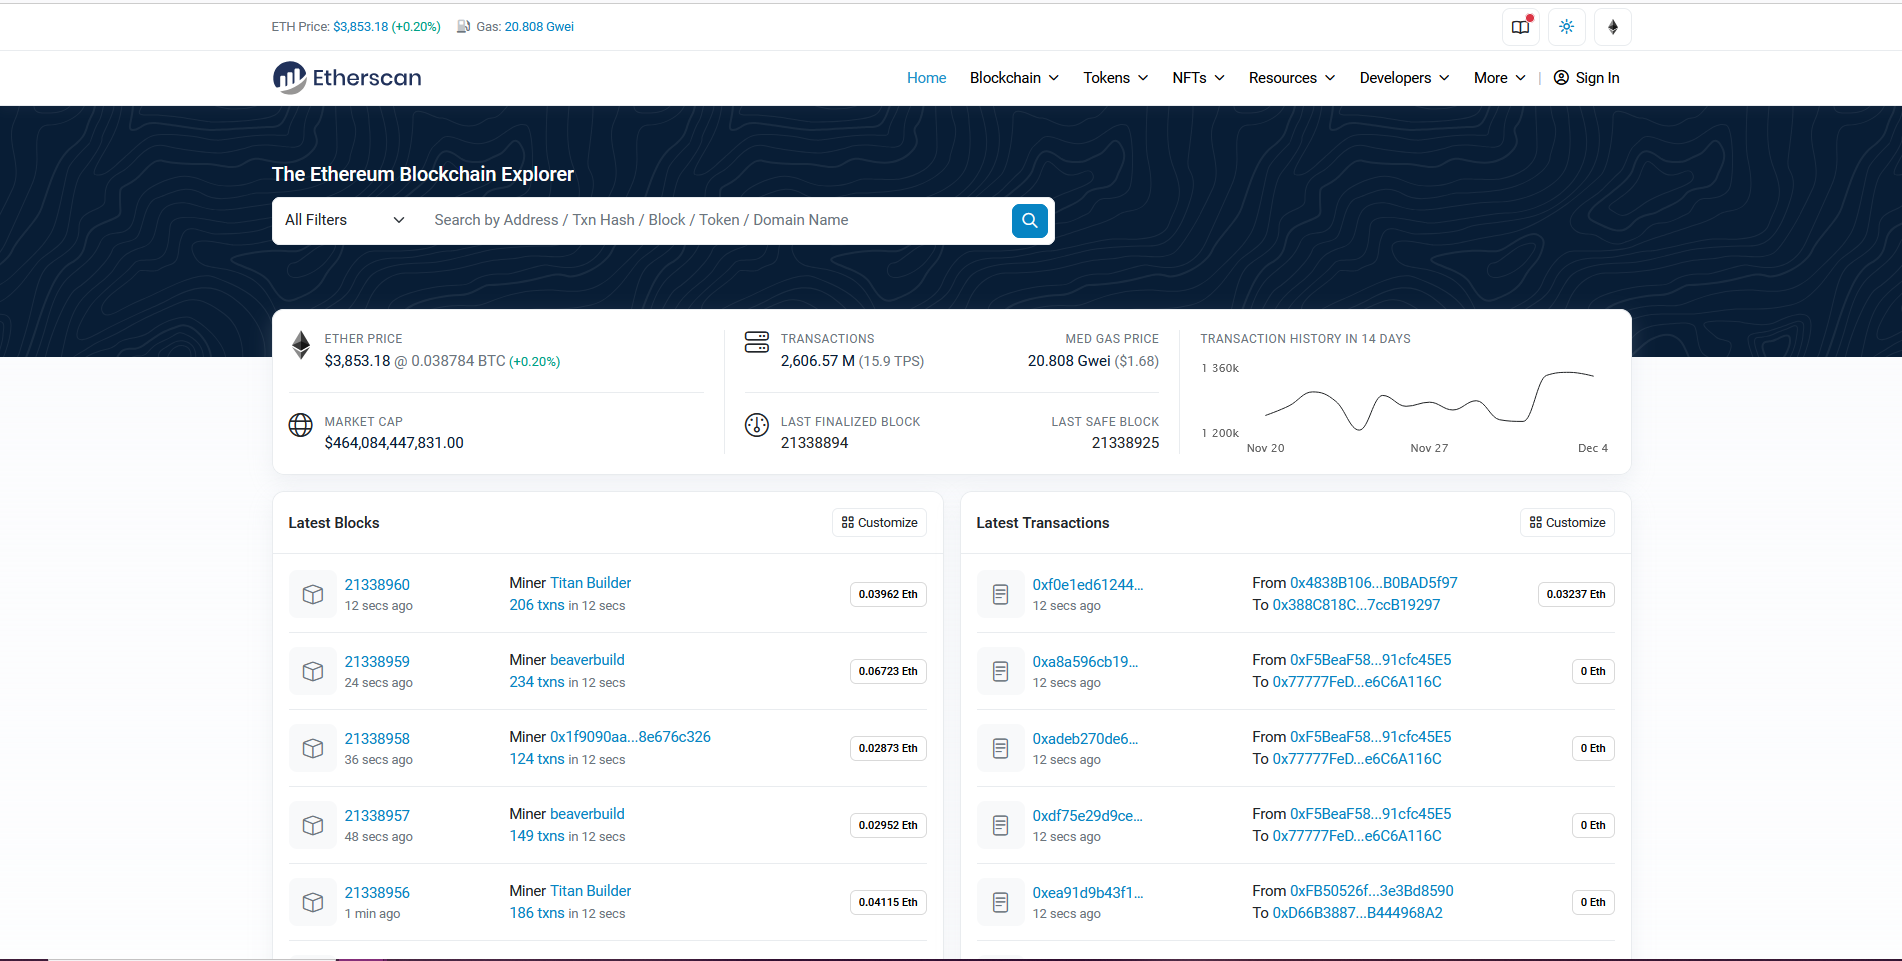
\includegraphics[width=0.8\linewidth]{./obrazy/Etherscan.png}
    \caption{Etherscan}
    \label{fig:Etherscan}
\end{figure}
W odpowiedzi na te braki dobrym pomysłem byłoby stworzenie platformy zapewniającej użytkownikom nie tylko dostęp do wiedzy, ale także pozwalającej na bezpośrednie sprawdzania danych z blockchainów, takich jak aktualne transakcje, stan kont oraz informacje o stanie sieci. Pomysł ten stał się podstawą do zdefiniowania tematu niniejszej pracy.


\section{Cel i zakres pracy}
Celem niniejszej pracy inżynierskiej jest zaprojektowanie i zaimplementowanie platformy internetowej przeznaczonej dla użytkowników kryptowalut i technologii blockchain. Ma ona służyć nie tylko poszerzaniu wiedzy, ale także otworzyć dostęp do funkcji pozwalających na bezpośrednie sprawdzanie danych z różnych sieci blockchain bez potrzeby korzystania ze specjalizowanych narzędzi przypisanych do poszczególnych sieci.

Platforma ma wspierać trzy główne blockchainy: Bitcoin, Ethereum i Solana, pozwalając użytkownikom na wybór interesującej ich sieci oraz uzyskanie dostępu do aktualnych danych na jej temat. W szczególności powinna ułatwić analizę różnic między blockchainami pod względem struktury bloków oraz funkcjonowania kont użytkowników, oferując funkcje do monitorowania i analizowanie bieżących danych. Dokładniej, platforma powinna umożliwiać:
\begin{itemize}
\item \textbf{przeglądanie szczegółowych informacji o wybranych blockchainach}, takich jak dane bloków, transakcji i kont; 
\item \textbf{bezpośrednie sprawdzanie danych z sieci blockchain} poprzez integrację z API, np.\ Alchemy (co pozwoli na weryfikację stanu kont, przeglądanie historii transakcji oraz monitorowanie stanu sieci  w czasie rzeczywistym, np.\ monitorowanie liczby aktywnych węzłów czy bieżącej opłaty transakcyjnej);
\item \textbf{symulację transakcji na blockchainie Solana}, co ułatwi użytkownikom zrozumienie procesu przesyłania środków w rzeczywistej sieci;
\item \textbf{dostęp do przewidywań cen kryptowalut z wykorzystaniem modeli sztucznej inteligencji}, co wyrobić ma dobre nawyki oraz pozwolić na lepsze planowanie inwestycji;
\item \textbf{konwersję walut tradycyjnych na kryptowaluty oraz odwrotnie}, co pozwoli na szybkie obliczenia związane z inwestycjami. 
\end{itemize}

Realizacja projektu wymaga zastosowania zaawansowanych technologii i narzędzi programistycznych, co nadaje pracy charakter inżynierski. Frontend platformy zostanie zbudowany w technologii React, co zapewni dynamiczny i responsywny interfejs użytkownika, umożliwiający łatwe przeglądanie danych oraz wykonywanie operacji. Backend, stworzony przy użyciu frameworka Spring Boot, będzie odpowiedzialny za integrację z zewnętrznymi API oraz przetwarzanie danych blockchainowych w sposób bezpieczny i wydajny. Wdrożenie platformy odbędzie się z wykorzystaniem rozwiązań chmurowych, takich jak Amazon Web Services (AWS), co zapewni elastyczność, skalowalność i niezawodność systemu.

Szczególny nacisk zostanie położony na bezpieczeństwo przetwarzania i przesyłania danych blockchainowych. Platforma będzie wykorzystywać szyfrowanie danych, co zapewni ochronę wrażliwych informacji użytkowników oraz ich transakcji. Dzięki temu użytkownicy będą mogli wykonywać operacje na blockchainie bez obaw o bezpieczeństwo swoich danych.

\section{Układ pracy}
Praca składa się z sześciu głównych rozdziałów. Pierwszy rozdział, Wstęp, wprowadza w tematykę pracy, przedstawiając ogólny zarys problematyki związanej z nauką technologii blockchain oraz dostępem do wielu danych w jednym miejscu. Zawiera również cel i zakres pracy oraz metodykę realizacji projektu. W rozdziale Analiza wymagań szczegółowo opisano założenia ogólne dotyczące zaprojektowanej platformy, integrację z API blockchainów oraz metody przechowywania danych. Omówiono również wymagania niefunkcjonalne, takie jak wydajność, bezpieczeństwo i skalowalność systemu. Implementacja koncentruje się na procesie budowy platformy, omawiając podział logiczny systemu na komponenty oraz opis interakcji między nimi. Przedstawiono również zastosowane technologie, w tym React, Spring Boot i Docker, oraz szczegóły konteneryzacji aplikacji. W rozdziale Testy aplikacji backendowej opisano jak aplikacja została przetestowana, tak aby zweryfikować poprawność działania poszczególnych komponentów systemu. Wdrożenie omawia szczegóły procesu uruchomienia systemu w środowisku produkcyjnym, uwzględniając konfigurację lokalną i chmurową, z wykorzystaniem Amazon Web Services (AWS), oraz zasady użytkowania aplikacji i zapewnienia jej bezpieczeństwa. W ostatnim rozdziale, Podsumowanie, przedstawiono osiągnięcia co udało się zrealizować w pracy. Ponadto, praca zawiera spis treści, spis rysunków, tabel oraz bibliografię, co zapewnia strukturę zgodną z wymaganiami formalnymi.